\documentclass[../main.tex]{subfiles}

\begin{document}

In questa parte considero come estrarre informazioni sulla struttura di equilibrio dalle frequenze dei modi osservati: modi distinti sono confinati in cavit\'a di profondit\'a diversa e le ampiezze di oscillazione hanno differente comportamento spaziale, \'e quindi possibile invertire il problema date le frequenze osservate per ricavare il profilo radiale di $(P,\rho,\Gamma_1)$.

Un'inversione indipendente dal modello \'e possibile utilizzando l'approssimazione asintotica, valida nelle regioni in cui le autofunzioni variano molto pi\'u rapidamente delle grandezze di equilibrio e che trascura la perturbazione del potenziale gravitazionale.
 
L'inversione del sistema completo di equazioni dei modi si effettua considerando le perturbazioni al MSS che danno un miglior accordo tra frequenze osservate e predette dal MSS: considero solo i termini lineari nelle perturbazioni e quindi le correzioni agli autovettori sono trascurate.

I risultati dell'inversione sismologica permettono di valutare l'accuratezza della struttura del \mss{} , in particolare del profilo radiale della velocit\'a del suono, della densit\'a e di $\Gamma_1$; inoltre, usando l'equazione di stato per esplicitare la dipendenza di $\Gamma_1$ da $Y$, \'e possibile ricavare l'abbondanza di elio nella zona convettiva $Y_{CZ}$.

\'E possibile ricavare le caratteristiche della base della zona convettiva, profondit\'a della zona convettiva $d_{CZ}=\rsun{}-R_{CZ}$, $\rho_b=\rho(R_{CZ})$, $c_s=c_s(R_{CZ})$, oltre a $Y_{CZ}$, con grande accuratezza.


{\let\clearpage\relax\let\cleardoublepage\relax \chapter{Inversione della legge di Duvall.}} % Inizio chapter "Inversione asintotica." senza nuava pagina

%Si ricava, usando le espressioni asintotiche \eqref{cowosc:main}, il profilo radiale della velocit\'a del suono indipendente dal modello solare e si determina l'effetto dell'evoluzione stellare sui modi p di basso ordine radiale.
%Considerando la differenza tra risultati relativi a diversi set di frequenze \'e possibile attenuare gli effetti degli errori sistematici dovuti alla descrizione asintotica.


L'inversione della legge di Duvall \eqref{eq:duvallexpli} permette di ricavare il profilo di $c_s(r)$ sulla base dei modi osservati, tuttavia le approssimazioni fatte introducono errori sistematici: per i modi pi\'u penetranti nell'interno solare la perturbazione del potenziale gravitazionale influenza sensibilmente $F(\frac{\omega}{L})$ mentre per modi confinati vicino alla superficie $\alpha$ dipende da l.


\section{Inversione analitica della velocit\'a del suono}

\begin{wrapfigure}[13]{r}{0.45\textwidth}
        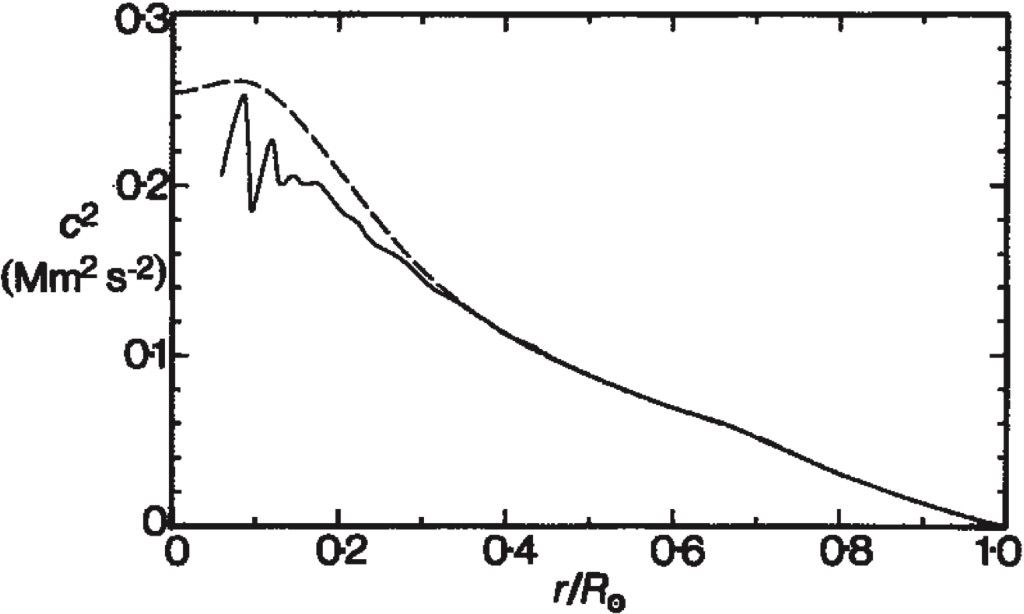
\includegraphics[width=0.44\textwidth,keepaspectratio]{soundspeed}
        \caption{Profilo radiale di $c_s^2$ determinato invertendo \eqref{eq:analinversionc} dalle frequenze dei modi osservate. Da \cite{christensen1985speed}.}\label{fig:soundspeedccm}
\end{wrapfigure}

L'equazione \eqref{eq:duvallf} pu\'o essere invertita analiticamente:
\begin{equation}
r=R\Exp{-\frac{2}{\pi}\int_{a_s}^a(w\expy{-2}-a\expy{-2})\expy{-\frac{1}{2}}\TDy{w}{F}\,dw}\label{eq:analinversionc}
\end{equation}

dove $a=\frac{c_s}{r}$.

Dall'equazione precedente, nota la funzione $F(w)$ dalle osservazioni, di ricavare $c_s(r)$ (vedi figura \ref{fig:soundspeedccm}). Il confronto tra $c_{sm}(r)$ calcolato tramite un modello solare e $c_{s0}(r)$ invertito usando l'equazione precedente per lo stesso modello mostra che l'errore sistematico dovuto alla tecnica di inversione nel range $0.4\leq x \leq 0.9$ \'e minore del $2.5\%$.


\section{Struttura dei modi penetranti nel core stellare}

La deviazione dalla \eqref{eq:freqequi} fornisce informazioni sull'evoluzione chimica del core di fusione: infatti estendendo ancora l'espansione di \eqref{eq:duvallf} si ha una misura della variazione di $c_s$ nel core della stella
\begin{equation}\label{eq:tassoul}
    d_{nl}=\nu_{nl}-\nu_{n-1,l+2}\approx-(4l+6)\frac{\Delta\nu}{4\pi^2\nu_{nl}}\int_0^R\frac{dc_s}{dr}\frac{dr}{r}
\end{equation}
La velocit\'a del suono \'e ridotta a causa dell'aumentare di $\mu$ durante la fusione di H in He durante l'evoluzione stellare: il centro solare \'e un minimo locale per la velocit\'a del suono e quindi, essendo il gradiente della velocit\'a del suono positivo, la parte centrale da un contributo sempre pi\'u negativo in \eqref{eq:tassoul} con l'evolversi della stella.

\section{Forma differenziale della legge di Duvall}

Considero l'effetto di perturbazioni del modello sulle frequenze dei modi introducendo nella legge di Duvall \eqref{eq:duvallexpli} perturbazioni nel profilo della velocit\'a del suono e in $\alpha$:
\begin{equation}
S_{nl}\frac{\delta\omega_{nl}}{\omega_{nl}}\approx H_1(\frac{\omega_{nl}}{L})+H_2(\omega_{nl})\label{eq:Dlinear}
\end{equation}

\begin{align}
&S_{nl}=\int_{r_t}^R(1-\frac{L^2c^2}{r^2\omega_{nl}^2})\expy{-\frac{1}{2}}\frac{dr}{c}-\pi\TDy{\omega}{\alpha}\\
&H_1(w)=\int_{r_t}^R(1-\frac{c^2}{r^2w^2})\expy{-\frac{1}{2}}\frac{\delta_rc}{c}\frac{dr}{c},\ H_2(\omega)=\frac{\pi}{\omega}\delta\alpha(\omega)
\end{align}

La funzione $S_{nl}$ \'e approssimabile con un temine proporzionale a $Q_{nl}$ (\cite{christensen1991solar}):
\begin{align}
&\frac{S_{nl}}{\tau_0}\approx Q_{nl}\intxt{con}
&\tau_0=\int_{0}^R\frac{dr}{c_s}
\end{align}

Le funzioni $H_1(\frac{\omega_{nl}}{L})$ e $H_2(\omega_{nl})$ possono essere ottenute separatamente attraverso fitting dei dati sperimentali: la prima caratterizza il contributo alle differenze nelle frequenze dei modi dovuto alle differenze del profilo radiale della velocit\'a del suono, la seconda alle diffenze nella regione vicino alla superficie.

\begin{wrapfigure}[29]{r}{0.45\textwidth}
        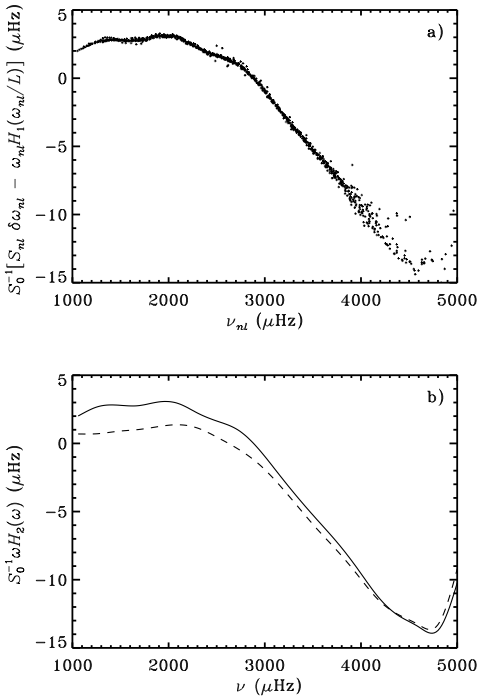
\includegraphics[width=0.44\textwidth,keepaspectratio]{H2dnd}
        \caption{a) Residuo della differenza di frequenze fra il sole e un modello senza diffusione a cui \'e stato sottratto $H_1$. b) Fit di $H_2$ linea continua e per contrasto fit di $H_2$ per differenze di frequenze tra Sole e modello con diffusione. Da \cite{dal03notes}.}\label{fig:H2dnd}
\end{wrapfigure}

La relazione \eqref{eq:Dlinear}, considerando che $1-\midfrac{L^2c^2}{r^2\omega^2}\approx1$ ad eccezione delle regioni vicino al punto d'inversione $r_t$, pu\'o essere approssimata da
\begin{equation}
\frac{\delta\omega}{\omega}\approx\frac{\int_{r_t}^{R}\frac{\delta_rc_s}{c_s}\frac{dr}{c_s}}{\int_{r_t}^R\frac{dr}{c_s}}
\end{equation}
Le differenze nella velocit\'a del suono nelle varie regioni influiscono sulle differenze nelle frequenze con un peso dato dal tempo impiegato da un'onda sonora ad attraversare la regione: le differenze nella regione vicino alla superficie dove $c_s$ \'e minore hanno un effetto relativamente grande sulle differenze di frequenza.

Una volta determinato $H_1$ le differenze nel profilo radiale di $c_s$ sono determinate tramite
\begin{equation}
\frac{\delta_rc_s}{c_s}=-\frac{2a}{\pi}\TDof{\ln{r}}\int_{a_s}^a(a^2-w^2)\expy{-\frac{1}{2}}H_1(w)\,dw
\end{equation}

%buon accordo range $0.2-095\ \rsun{}$.
%Le differenze in $c_s$ corrispondono a errori nel modello in $\frac{T}{\mu}$ minori del $2\%$.
%confronto diffusion no diffusion model.
%separation opacity uncertainties from effects of diffusion and settling.
%Inversione di $H_2$ ?? H He ionization zones.

La funzione $H_2$ \'e determinata dalla regione sotto la fotosfera. \cite{chr92phase}, analizzando la relazione tra $H_2(\omega)$ e le differenze in $c_s(r)$ e $\Gamma_1$ nelle regioni esterne, hanno visto che discrepanze pi\'u vicino alla superficie generano una componente lentamente oscillante in $H_2(\omega)$ e la ''frequenza'' aumenta con l'aumentare della profondit\'a. \'E inoltre possibile indagare l'andamento di $\Gamma_1$ nella regione di seconda ionizzazione di He e pi\'u in generale il comportamento di $H_2(\omega)$ nelle zone di ionizzazione di H e He consente un'analisi dell'equazione di stato e determinazione dell'abbondanza di elio nella zona convettiva. In figura \ref{fig:H2dnd} si mostra le differenze nelle frequenze tra il Sole ed un modello che non considera la diffusione degli elementi: l'andamento oscillatorio della linea continua nel pannello b \'e dovuto alla differenza nell'abbondanza di idrogeno negli strati superficiali.

% Dalsnotes 7.155, fig 7.15
%vedi relative sharp variations in $\Gamma_1$ in He second ionization zone Influence of the upper layers of the sun on the p-mode frequencies


{\let\clearpage\relax\let\cleardoublepage\relax \chapter{Inversione non asintotica.}} % Inizio chapter "Inversione non asintotica." senza nuava pagina

La soluzione del problema inverso per il sistema completo di equazioni si basa sulla linearizzazione delle variazioni attorno ad un modello di cui siano calcolabili le autofunzioni dell'operatore $L$ definito in \eqref{eq:variational}.

Utilizzo la formula \eqref{eq:variational} specializzata al problema dell'inversione delle differenze $\delta\omega_{nl}=\omega_{\odot}-\omega_{Mod}$ fra frequenze osservate e predette da un modello. Per l'inversione della struttura idrostatica si ha:
\begin{align}
&\frac{\delta\omega_{nl}}{\omega_{nl}}=\int_0^R[K^{nl}_{c^2,\rho}(r)\frac{\delta_rc^2}{c^2}(r)+K^{nl}_{\rho,c^2}(r)\frac{\delta_r\rho}{\rho}(r)]\,dr+I_{nl}\expy{-1}F_{Surf}(\omega_{nl})+\sigma_i\label{eq:invstructure}\intxt{dove $\sigma_i$ \'e l'incertezza sulle frequenze osservate e}
&\frac{\delta_rc^2}{c^2}(r)=\frac{[c_{\odot}^2(r)-c_{mod}^2(r)]}{c^2(r)},\ \frac{\delta_r\rho}{\rho}(r)=\frac{[\rho_{\odot}(r)-\rho_{mod}(r)]}{\rho(r)}
\end{align}

E quindi si determinano attraverso procedure numeriche le correzioni alla struttura del modello sulla base delle differenze tra frequenze dei modi. Il peso che una perturbazione ha sulla differenze in frequenza \'e determinato dalle autofunzioni dei modi calcolate tramite un modello solare.
%Asymptotic approximation for radial eigenfunction (integral equation connectin sound speed $c(r)$ to $\Omega_{nl}$) is inadequate (especially in deep interior)

In \ref{fig:deltacwu} la banda chiara attorno allo zero, che indica il modello solare in perfetto accordo con le osservazioni sismologiche, mostra l'incertezza nell'inversione della velocit\'a del suono; essa \'e dovuta a

\begin{itemize}

\item Incertezze nelle frequenze dei modi osservate. Oltre all'incertezza statistica propria del determinato strumento \'e possibile valutare gli effette di eventuali errori sistematici confrontando i risultati dell'inversione per set di frequenze ottenute con strumenti diversi: la differenza nella velocit\'a del suono \'e minore di $0.02\%$.

\begin{workout}[Accuratezza frequenze osservate]
!
\end{workout}


\item Incertezze inerenti la tecnica di inversione.

\item Incertezze legate alla dipendenza da un modello solare per il calcolo dei kernel in \eqref{eq:invstructure}, \eqref{eq:invdGammadrho}, \eqref{eq:splitfreqrotation}.

\end{itemize}

\begin{workout}[incertezze]
[quantificare errori dovuti a errori misura frequenze e dipendenza modello solare dei kernel]
I risultati dell'inversione sono affetti da errori sistematici introdotti dalla procedura di inversione ([vedi effetti risoluzione finita sunto pg 1098 $\S 10$ pbp 2000 e DDFR97]).
[quantificare: effetti risoluzione kernel e tecniche numeriche (regolarizzazione)]
\ref{fig:deltacwu}
\end{workout}

\section{Tecniche di inversione numeriche.}
%vedi JCD 2002 pg 25-32

Elenco alcune tecniche numeriche usate. Considero per sempicit\'a una sola funzione da invertire $\frac{\delta f}{f}$, legata a $\delta\omega$ da \eqref{eq:variational}.

\begin{workout}[Forma splitting frequenze: principio variazionale]

$\midfrac{\delta\omega}{\omega}$ da \eqref{eq:variational}: forma esplicita dipende dalle quantit\'a da invertire.

Due funzioni indipendenti di $\rho$, $P$, $\Gamma_1$ determinano i modi di oscillazione quindi indico con $\frac{\delta f_1}{f_1}$ e $\frac{\delta f_2}{f_2}$

\end{workout}


\begin{workout}[Inversione RLS/$\chi^2$ vs SOLA]

Due funzioni indipendenti di $\rho$, $P$, $\Gamma_1$ determinano i modi di oscillazione quindi indico con $\frac{\delta f_1}{f_1}$ e $\frac{\delta f_2}{f_2}$

\end{workout}

\subsection{RLS}

\begin{workout}[parametrizzo incognite tramite polinomi: legendre e cubic spline]

Usando la tecnica del minimo $\chi^2$ regolarizzato si parametrizzano le funzioni incognite $\frac{\delta f_1}{f_1}$, $\frac{\delta f_2}{f_2}$ e $F_{Surf}$. Attraverso la tecnica dei minimi quadrati si determinano i coefficienti dei polinomi.

\end{workout}

Usando la tecnica del minimo $\chi^2$ regolarizzato si parametrizza la funzione incognita $\frac{\delta f}{f}$ tramite funzioni di base opportune.

La funzione da minimizzare \'e
\begin{equation}
Y=(N-N_p)\chi^2+\alpha N\int_0^1(x\TDof{x}\frac{\Delta f}{f})^2\,dx\label{eq:minimizerls}
\end{equation}
con
\begin{equation}
\chi^2=\frac{1}{N-N_p}\sum_{\alpha=1}^N(\frac{\delta\omega_{obs}-\delta\omega_{fit}}{\sigma})^2_{\alpha}
\end{equation}
N indica il numero totale di modi $\alpha$, $N_p$ il numero di parametri da determinare, $\Delta\nu_{fit}$, ricavato tramite \eqref{eq:variational}, contiene la funzione incognita opportunamente parametrizzata; il secondo addendo del lato destro di \eqref{eq:minimizerls} \'e introdotto per ridurre oscillazioni indesiderate nel risultato dell'inverisone con $\alpha$, parametro di regolarizzazione, scelto opportunamente.

\begin{workout}[Incertezze inerenti RLS]
parametro regolarizzazione, numbers of bins, number of legendre polynomials
\end{workout}
%Determinazione incertezza.
%(Dziembowski90, Antia Basu 94), (JCD90).

\begin{workout}[Inversion: forma esplicita delta freq]
ed \'e dato da \eqref{eq:diffthermo} o \eqref{eq:invstructure}, $\sigma$ \'e l'errore osservativo
\end{workout}

\subsection{Subtractive Optimally Localized Averaging}

\begin{workout}[Risoluzone: largezza dei kernel]
Risoluzione inversione \'e caratterizzata dalla larghezza dei kernel: il valore della grandezza a $r_0$ \'e una media sulla regione in cui il kernel ha il valore massimo.
\end{workout}

\begin{workout}[OLA]
$\mathcal{K}(r,r_0)\approx\delta(\vec{r}-\vec{r}_0)$, $\int_0^R\mathcal{K}(r,r_0)\,dr=1$
\end{workout}

\begin{workout}[SOLA $f_i$ / OLA]

Per determinare in generale la funzione $\frac{\delta f_1(r)}{f_1(r)}$ scelgo i $c_i(r_0)$ tali che $\sum c_i(r_0)\frac{\delta\omega_i}{\omega_i}$ fornisca una media del valore di $\frac{\delta f_1(r)}{f_1(r)}$ in $r=r_0$:

\begin{align*}
&\sum_ic_i(r_0)\frac{\delta\omega_i}{\omega_i}=\int_0^R\sum_ic_i(r_0)K_{1,2}^i(r)\frac{\delta f_1(r)}{f_1(r)}\,dr+\int_0^R\sum_ic_i(r_0)K_{2,1}^i(r)\frac{\delta f_2(r)}{f_2(r)}\,dr+\sum_ic_i(r_0)\frac{F_{Surf}(\omega_i)}{\omega_i}
\end{align*}

Il primo termine approssima il valore di $\frac{\delta f_1}{f_1}$ pesato dal kernel $\mathcal{K}(r,r_0)=\sum_ic_i(r_0)K_{1,2}^i(r)$, il secondo tiene conto dell'influenza che hanno le discrepanze della seconda funzione su quelle della funzione che abbiamo scelto di invertire pesate da $\mathcal{L}_{21}(r_0,r)=\sum_ic_i(r_0)K_{21}^i(r)$, il terzo \'e il termine di superficie: i coefficienti $c_i(r_0)$ sono scelti in maniera da riprodurre la funzione target, minimizzare la contaminazione delle $\frac{\delta f_2}{f_2}$ via $\mathcal{L}_{21}$ e il rumore.

\end{workout}

Scelgo dei coefficienti $c_i(r_0)$ tali che $\sum c_i(r_0)\frac{\delta\omega_i}{\omega_i}$ fornisca una media del valore di $\frac{\delta f(r)}{f(r)}$ in $r=r_0$:

\begin{equation}\label{eq:SOLAfmean}
\sum_ic_i(r_0)\frac{\delta\omega_i}{\omega_i}=\int_0^R\sum_ic_i(r_0)K^i(r)\frac{\delta f(r)}{f(r)}\,dr=\exv{\frac{\delta f(r_0)}{f(r_0)}}
\end{equation}

e i coefficienti $c_i(r_0)$ sono determina minimizzando la funzione

\begin{equation}\label{eq:SOLAcir0min}
\int_0^R[\mathcal{K}(r_0,r)-\mathcal{T}(r_0,r)]^2\,dr+\mu\sum_i\sigma_ic_i(r_0)c_j(r_0)\\
\end{equation}
con $\mathcal{K}(r_0,r)=\sum_ic_i(r_0)K^i(r)$ e la funzione target $\mathcal{T}(r_0,r)$, la cui larghezza \'e anch'essa parametro del fit, determina la natura precisa della localizzazione.

La larghezza finita di $\mathcal{K}(r_0,r)$ determina il valor medio di $\frac{\delta f}{f}$ in intorno di $r_0$ e ci\'o causa una differenza sistematica  dal valore effettivo in $r_0$: per $c_s$ l'errore \'e minore del $0.03\%$ e le regioni pi\'u afflitte sono la base della zona convettiva, per la rapida variazione di $\frac{\delta c_s}{c_s}$ e la regione centrale, per il ridotto numero di modi che penetrano in questar zona.


\begin{errata}[Funzione da minimizzare in SOLA: manca la funzione terget]
I parametri si trovano minimizzando
\begin{align*}
&\int(\sum_ic_iK_{12}^i)^2\,dr+\beta\int(\sum_ic_iK_{21}^1)^2\,dr+\mu\sum_{ij}c_ic_jE_{ij}
\end{align*}
$\beta$ \'e un parametro per il contributo del secondo termine, $E$ \'e una matrice che rappresenta le incertezze sulle frequenze osservate.

\end{errata}

Illustro la tecnica SOLA per determinare $\frac{\delta_rc^2}{c^2}$: si formano delle combinazioni lineari di $\frac{\Lvar{\omega_i}}{\omega_i}$ pesate da coefficienti $c_i(r_0)$ tali che $\frac{\Lvar{c^2}}{c^2}$ sia centrato attorno $r_0$ e che gli altri termini in \eqref{eq:invstructure} siano soppressi, queste compongo un averaging kernel $\mathcal{K}_{c^2,\rho}(r_0,r)=\sum_ic_i(r_0)K_{c^2,\rho}^i(r)$, con $\int_0^R\mathcal{K}(r_0,r)\,dr=1$.

Determino i coefficienti minimizzando l'espressione
\begin{equation}
\int_0^R[\mathcal{K}_{c^2,\rho}(r_0,r)-\mathcal{T}(r_0,r)]^2\,dr+\beta\int_0^R\mathcal{L}_{\rho,c^2}(r_0,r)\,dr+\mu\sum_i\sigma_ic_i(r_0)c_j(r_0)
\end{equation}
dove il kernel cross-term
\begin{equation}
\mathcal{L}_{\rho,c^2}(r_0,r)=\sum_ic_i(r_0)K_{\rho,c^2}^i(r)
\end{equation}
controlla i contributi indesiderati di $\frac{\delta_r\rho}{\rho}$.

%Il primo termine approssima il valore di $\frac{\delta c^2}{c^2}$ pesato dal kernel $\mathcal{K}(r,r_0)=\sum_ic_i(r_0)K_{c^2,\rho}^i(r)$, il secondo tiene conto dell'influenza che hanno le discrepanze della seconda funzione su quelle della funzione che abbiamo scelto di invertire pesate da $\mathcal{L}_{\rho,c^2}(r_0,r)=\sum_ic_i(r_0)K_{\rho,c^2}^i(r)$, il terzo \'e il termine di superficie: i coefficienti $c_i(r_0)$ sono scelti in maniera da riprodurre la funzione target, minimizzare la contaminazione delle $\frac{\delta \rho}{\rho}$ via $\mathcal{L}_{\rho,c^2}$ e il rumore.

\begin{comment}
\section{risultati inversione}
[reminder: EOS dependence:LInantiabasu07]
[reminder: errori: sperimentali/numerici/modello per inversione $(\rho,Y)$, $(\rho,\Gamma_1)$]
%% discrepanza densita e velocita suono con metallicita riviste
%[figure inversione al variare dei parametri solari da \cite{boothroyd2003our}]
[reminder: errori: sperimentali/numerici/modello per inversione $(\rho,c^2)$]
\begin{wraptable}{r}{5.5cm}
\begin{tabular}{|cccc|}
&$\Delta_{exp}$&$\Delta_{num}$&$\Delta_{mod}$\\
$\frac{\delta c}{c}$&$0.02\%$&&\\
$\frac{\delta\rho}{\rho}$&&&\\
\end{tabular}
\end{wraptable}
\end{comment}

\section{Inversione della rotazione.}

%Deviazioni dalla simmetria sferica introducono una dipendenza delle frequenze dei modi da m. L'effetto della rotazione \'e descritto al primo ordine (in $\Omega$) da 
%Spesso \'e impossibile misurare lo splitting in m quindi si parametrizzano le frequenze nel multipletto $(n,l)$ tramite:
%\begin{equation}
%\nu_{nlm}=\nu_{nl0}+\sum_{j=1}^{j_{\max}}a_j(n,l)\pol_j^{(l)}(m)\label{eq:freqmulti}
%\end{equation}
%[fitting power spectra to measure splitting coefficients]
%Le deviazioni dalla simmetria sferica causano uno splitting delle frequenze: rappresento un multipletto di frequenze tramite espansione con base di polinomi appropriata (solitamente si usano i polinomi di Legendre)
%\begin{equation}
%\nu_{nlm}=\nu_{nl0}+\sum_{j=1}^{j_{\max}}a_j(n,l)\pol_j^{(l)}(m)\label{eq:freqmulti}
%\end{equation}
%e ricavo i coefficienti tramite fit con le frequenze osservate; i coefficienti dispari contengono il contributo della rotazione al termine lineare, i coefficienti pari effetti delle asfericit\'a nella struttura solare e effetti quadratici della rotazione.

\begin{figure}[!ht]
\centering
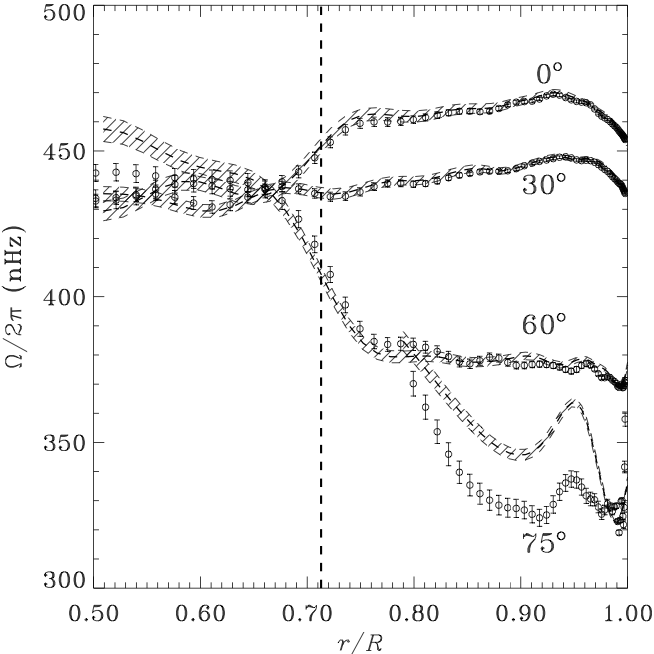
\includegraphics[keepaspectratio,width=0.8\textwidth]{invertedrotation}
\caption{Inversione della velocit\'a di rotazione a diverse latitudini. La linea verticale tratteggiata indica la base della zona convettiva. Da \cite{chr02helioseismology}.}
\end{figure}

Per inversione 2D, cio\'e che considera la dipendenza generica $\Omega(r,\theta)$, si esprimono direttamente le differenze in frequenze:
\begin{equation}
\omega_{nlm}-\omega_{nl0}=m\int_0^R\int_0^{\pi}K_{nlm}(r,\theta)\Omega(r,\theta)r\,dr\,d\theta\label{eq:invrot2D}
\end{equation}

mentre nel caso si abbiano i coefficienti $a_{2s+1}$, scrivo la velocit\'a angolare nella forma
\begin{equation}
\Omega(r,\theta)=\sum_{s=0}^{s_m}\Omega_{s}(r)\psi_{2s}(\cos{\theta})\label{eq:angularv15}
\end{equation}
dove $\psi_{2s}$ sono polinomi opportuni.

Esiste una funzione opportuna $K_{nls}^{s}(r)$ tale che
\begin{equation}
2\pi a_{2j+1}(n,l)=\int_0^R\int_0^{\pi}K_{nls}^{s}(r)\Omega_s(r)\,dr
\end{equation}
e quindi \'e possibile determinare $\Omega_s(r)$.
%2\pi a_j(n,l)=\sum_m\gamma_j(l,m)(\omega_{nlm}-\omega_{nl0}),\ 
%2\pi a_{2j+1}(n,l)=\int_0^R\int_0^{\pi}K_{nlj}^{(a)}(r,\theta)\Omega(r,\theta)r\,dr\,d\theta
%&\omega_{nlm}-\omega_{nl0}=m\int_0^R\int_0^{\pi}K_{nlm}(r,\theta)\Omega(r,\theta)r\,dr\,d\theta
%&\omega_{nlm}=\omega_{nl0}+2\pi\sum_{j=1}^{j_{max}a_j(n,l)\mathcal{P}_j^{(l)}(m)}
%$\Delta\omega$ e $a_j$ sono legatoi da dipendenza lineare.
%{infered angular velocity $\bar{\Omega}(r_0,\theta_0)$ is linearly related to data:}
%\bar{\Omega}(r_0,\theta_0)=\int_0^{\pi}\int_0^R\mathcal{K}(r,\theta,r_0,\theta_0)\Omega(r,\theta)r\,dr\,d\theta
%Per investigare la dipendenza $\Omega(r,\theta)$ devo considerare le $2l+1$ frequenze.
%latitudinal shear causa una deviazione da frequenze equispaziate.


{\let\clearpage\relax\let\cleardoublepage\relax
\chapter{Vincoli al modello solare dalle osservazioni sismologiche.}%%chapter: vincoli al modello solare: HCSM.
}

%\section{Osservabili sismologiche - approssimazione di scaling??}

\begin{figure}[!ht]%{r}{0.5\textwidth}
        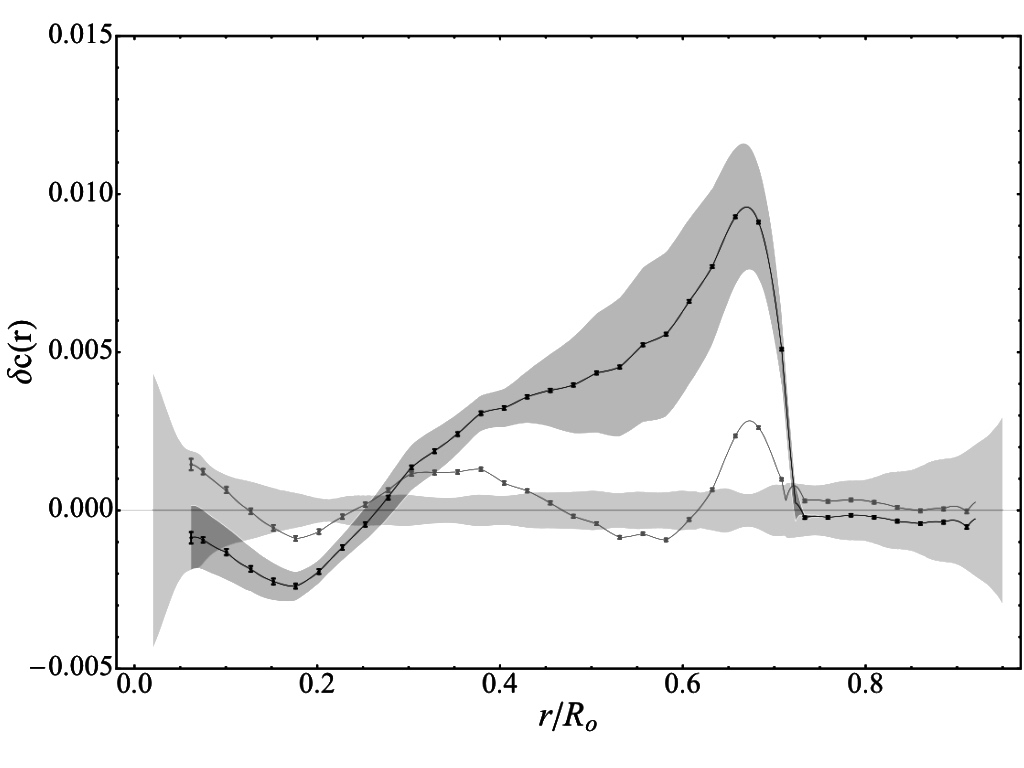
\includegraphics[width=0.9\textwidth,keepaspectratio]{deltacwu}
        \caption{Differenza relativa nel profilo di $c_s$ risultanei dall'inversione delle differenze in frequenza tra Sole e modello: la linea chiara si riferisce alle frequenze di un modello con composzione GS98, la linea scura a composizione AGSS09. La banda chiara mostra l'errore inerente l'inversione eliosismologica, la banda scura l'incertezza a $1\sigma$ sul profilo di $c_s$ predetto dal modello. Da \cite{villante2014chemical}.}\label{fig:deltacwu}
\end{figure}

\begin{table}[!ht]%{r}{0.7\textwidth}

\pgfplotstabletypeset[
math/.style={%
        preproc cell content/.append style={/pgfplots/table/@cell content/.add={$}{$}},
    },
every head row/.style={
 before row={\toprule
 %&\multicolumn{4}{c|}{Primordiale}
 },
 every last row/.style={after row=\bottomrule},
 after row={\midrule}
},
every last row/.style={after row=\bottomrule},
every first column/.style={column type/.add={|}{}},
every last column/.style={column type/.add={}{|}},
%columns/0/.style = {column type/.add={|}{}},
display columns/0/.style={column name={Composizione}},
display columns/1/.style={column name={$Z/X$}},
display columns/2/.style={column name={$R_{CZ}$}},
display columns/3/.style={column name={$Y_{CZ}$}},
display columns/4/.style={column name={$Y_0$}},
create on use/comp/.style={create col/set list={
inversione,GS98,AGS05,AGSS09,C+11}},
columns/comp/.style = {column type/.add={|}{}},
columns/comp/.style={string type},
columns/ZX/.style={string type},
columns/ZX/.append style={math},
columns/RCZ/.style={string type},
columns/RCZ/.append style={math},
columns/YCZ/.style={string type},
columns/YCZ/.append style={math},
columns/Y0/.style={string type},
columns/Y0/.append style={math},
columns={comp,ZX,RCZ,YCZ,Y0},
%/pgf/number format/precision=4
     ]{CZvsZ.txt} %%%
     \caption{Caratteristiche della zona convettiva: confronto tra valore eliosismologico e valore ricavato da modello solare con diverse metallicit\'a del raggio della base della zona convettiva $R_{CZ}$, dell'abbondanza di elio superficiale $Y_{CZ}$ e dell'abbondanza di elio primordiale. Da \cite{basu2016global}.}
\label{tab:CZZvar}
\end{table}

L'inversione di $c_s$ o $\rho$ mostra se un modello solare riproduce accuratamente la posizione della base della zona convettiva in quanto nella zona convettiva si ha gradiente adiabtico maggiore del gradiente radiativo; diminuzione di opacit\'a, nel caso determinata da una minore metallicit\'a, sposta la base della zona convettiva pi\'u in alto come da tabella \ref{tab:CZZvar}.

La figura \ref{fig:deltacwu} mostra che un modello solare con composizione GS98, meno accurata di AGSS09, riproduce il profilo di $c_s$ in maniera pi\'u accurata: ci\'o pu\'o indicare un'opacit\'a da incrementare nel modello. Analogamente la diminuzione dell'opacit\'a diminuisce il gradiente termico nella regione radiativa quindi a pari luminosit\'a si ha un contenuto di idrogeno maggiore.


\begin{comment}
Opacity changes affect structure radiative interior and position of $R_{cz}$
Equation of state depends on number of free particle per unit volume - number density of heavy elements is two order of magnitude smaller than that of He, H: small effect on pressure.
Ionization os elements causes $\Gamma_1$ to decrease in ionization zone.
The effect of Z on convection zone is due to effect on EOS.
CNO cycle increase vs opacity increase: vedi tab.12 bahcall06
\end{comment}
%[RMS sound speed difference: dominated by contrib from region where Z influence opacity]
%Region $R\geq0.45$: sources of opacity are BF transition, in inner regions electron scattering and ff transitions.

%(Vedi: \cite{bah04accurately})
%Sotto la zona convettiva $\Gamma_1=\frac{5}{3}$ con accuratezza migliore di \num{e-3}. L'inversione sismologica \'e accurata: $\frac{\Delta u}{u}\leq5 \permil$. Dalla conoscenza di $u_{\odot}$ si ricava il profilo radiale della velocit\'a del suono tramite $c_s^2=\Gamma_1 u$.
% Vedi H,SManf scilla pg 11-12
%Le propriet\'a di questa regione sono determinate dall'opacit\'a e quindi, nella misura in cui \'e possibile combinare le differenze nei modi per cancellare il contributo della zona convettiva e considerare il contributo di $\frac{\Lvar{L}}{L}$ una piccola correzione, come accade fuori dalla regione di produzione di energia, \'e possibile studiare gli effetti delle variazioni di opacit\'a sui modi.
%La quantit\'a da determinare \'e quindi
%\begin{equation}
%\frac{\delta\kappa}{\kappa}=\frac{\Lvar{\kappa}}{\kappa}+\Dcvar{\PDly{\rho}{\kappa}}{T}+\frac{\Lvar{T}}{T}\Dcvar{\PDly{T}{\kappa}}{\rho}
%\end{equation}
%dove $\frac{\Delta\kappa}{\kappa}$ rappresenta la correzione a $\kappa(\rho,T)$ a densit\'a, temperatura e composizione fissate.
%[vedi fig 11/12 \cite{ell95opacity} ??]
%{Core di fusione $x<0.2$.}
%Vedi \cite{ell98relativistic}
%Inversione di $(\delta\Gamma_1)_{int}$ mostra la necessit\'a di tener conto degli effetti relativistici per gli elettroni, che nel core solare hanno energia termica \SI{1.35}{\kilo\ev} approx $0.3\%$ of $m_e$).
%\begin{align}
%&\frac{\Lvar{\Gamma_1}}{\Gamma_1}\approx-\frac{2+2X}{3+5X}T&\intertext{dove T \'e in unit\'a di $\frac{m_ec^2}{k}$}\nonumber
%\end{align}
%[\cite{ell98relativistic} fig.3 ].
%[Solar neutrino deduced from solar seismic model]

\begin{comment}
Oltre a determinare il valore sismologico corretto delle grandezze meccaniche del modello solare si pu\'o stabilire il range dei parametri del SSM compatibili con le frequenze osservate: si approssima localmente una dipendenza della grandezza $Q$ dai parametri della forma $\frac{Q}{Q_{MSS}}=(\frac{P}{P_{MSS}})\expy{\alpha_{QP}}$ quindi si determina il range dei parametri $p_i=\frac{P^i}{P_{MSS}^i}$ compatibile con $\Omega_i\pm\Delta\Omega_i$, in particolare si usano le grandezze sismologiche pi\'u accurate $Y_{ph},\ R_b,\ \rho_b$.
La temperatura centrale dipende principalmente dall'opacit\'a e dal rapporto $\frac{Z}{X}$. Nella regione centrale si determina
\begin{align}
&R_b=R_{b,MSS}z\expy{-0.046}k\expy{-0.0084}\\
&\rho_b=\rho_{b,MSS}z\expy{0.47}k\expy{0.095}\\
&Y_{ph}=Y_{ph,MSS}z\expy{0.31}k\expy{0.61}&\intertext{dove k e z si riferiscono a opacit\'a e rapporto metalli/idrogeno.}\nonumber
\end{align}
Il valore ottimale dei parametri $(k,z)$ si determina minimizzando
\begin{equation}
\chi^2(z,k)=\sum_i(\frac{Q_{\odot i}-Q_i(z,k)}{\Delta Q_i})^2
\end{equation}
quindi per la temperatura centrale del Sole si ha 
\begin{equation}
T_{ES}=T_{MSS}(\frac{Y_{ph\odot}}{Y_{ph,MSS}})\expy{0.2}=\SI{1.587e7}{\kelvin}(\pm1.4\%)
\end{equation}
\end{comment}


%\begin{workout}[modello solare sismologico]
%Same structure equations of SSM but input parameters choosen as best fit helioseismic observable
%\end{workout}
%Indico con $Q(P)$ e $Q_{\odot}$ i valori di una grandezza Q determinati tramite un modello solare, funzione dei parametri del modello, e risultanti dalle correzioni sismologiche a quest ultimi  
%\begin{equation}
%&Q_{\odot}=Q(P)+q(\omega)
%\end{equation}
%\subsection{Zona convettiva}
%[accuratezza inversione $R_b$, $Y_{ph}$, $\rho_b$]
%Le osservabili sismologiche che caratterizzano la zona convettiva sono $R_b$, $Y_{ph}$ e $c_b$, $\rho_b$.
%\begin{itemize}
%\item L'abbondanza di elio \'e determinata da varii autori in un range $Y_{ph}=\numrange{0.226}{0.260}$.
%Il valore di $Y_{ph}$ inferiore di \numrange{0.27}{0.28}, richiesto per calibrare i modelli con la luminosit\'a attuale, conferma l'importanza della diffusione dell'elio verso il centro di gravit\'a.  
%\item Profondit\'a della zona convettiva.
%\begin{align*}
%&\frac{R_b}{\rsun{}}=\numrange{0.710}{0.716}\\
%&c_b=\SIrange{0.221}{0.225}{\mega\meter\per\second}
%\end{align*}
%\item Determinati tramite inversione il profilo radiale di u e $R_b$ si determina anche la densit\'a della base della zona convettiva:
%\begin{equation*}
%\rho_b=\SIrange{0.185}{0.199}{\gram\per\cubic\cm}
%\end{equation*}  
%\end{itemize}
%[\cite{deg97helioseismology} fig.3]
%\subsection{Reazioni nucleari}
%[figure inversione al variare dei parametri solari da \cite{boothroyd2003our}]


\end{document}